\chapter{Detalii de implementare}

Scopul extensiei create este de prelua un fișier PDF încărcat de profesor într-un formular din Moodle și de a genera automat module de învățare și teste grilă, teste cu patru variante de
răspuns și doar una corectă, pe baza informațiilor din fișier. Mediul de dezvoltare folosit este XAMPP, cu un server Apache, limbajul de programare PHP, o bază de date MariaDB, și
platforma Moodle instalată local. Generarea conținutului educațional pe baza materialului încărcat se face cu ajutorul API-ului Gemini de la Google, care oferă un model de inteligență 
artificială capabil să extragă și să reformuleze text pentru a genera module de învățare și să creeze întrebări cu un singur răspuns corect pentru testele ce faciliteaza trecerea individului 
la următorul nivel.  

\section{Arhitectura generală}

Arhitectura sistemului utilizează modelul client-server. Clientul este reprezentat de interfața Moodle, iar aceasta diferă în funcție de rolul utilizatorului. Pentru profesor, extensia va 
fi vizibilă sub forma unei activități Moodle și va putea fi adăugata ca orice altă activitate, cum ar fi Quiz, Lecție sau orice altă activitate preinstalată de configurația standard. 
După selectarea extensiei, profesorul va avea parte de un formular unde poate încărca documentul în format PDF, iar extensia va crea automat modulele în urma completării acesteia. 
După generarea modulelor profesorul selectează dacă le salvează sau le generează încă o dată. În urma salvării acestora, profesorul le poate vizualiza și este informat de progresul studenților 
ce au inceput această activitate, printr-un tabel unde este trecut numele studentului, modulul la care se află și ora la care a început modulul. Pentru student, interfața permite începerea
activității, unde studentul susține un test pentru a de la ce modul este asignat pentru a-și începe studiul, vizualizarea modulului de învățare curent și a testului generat pe baza căruia 
îi este facilitată trecerea la următorul modul. Serverul este aplicația Moodle încărcată local pe care este instalată extensia. Backend-ul extensiei se ocupă cu preluarea 
fișierului PDF, gestionarea permisiunilor de acces, încărcarea informațiilor în baza de date și comunicarea cu API-ul Gemini, folosit pentru generearea conținutului din cadrul modulelor și 
a testelor.

\begin{figure}[ht]
    \centering
    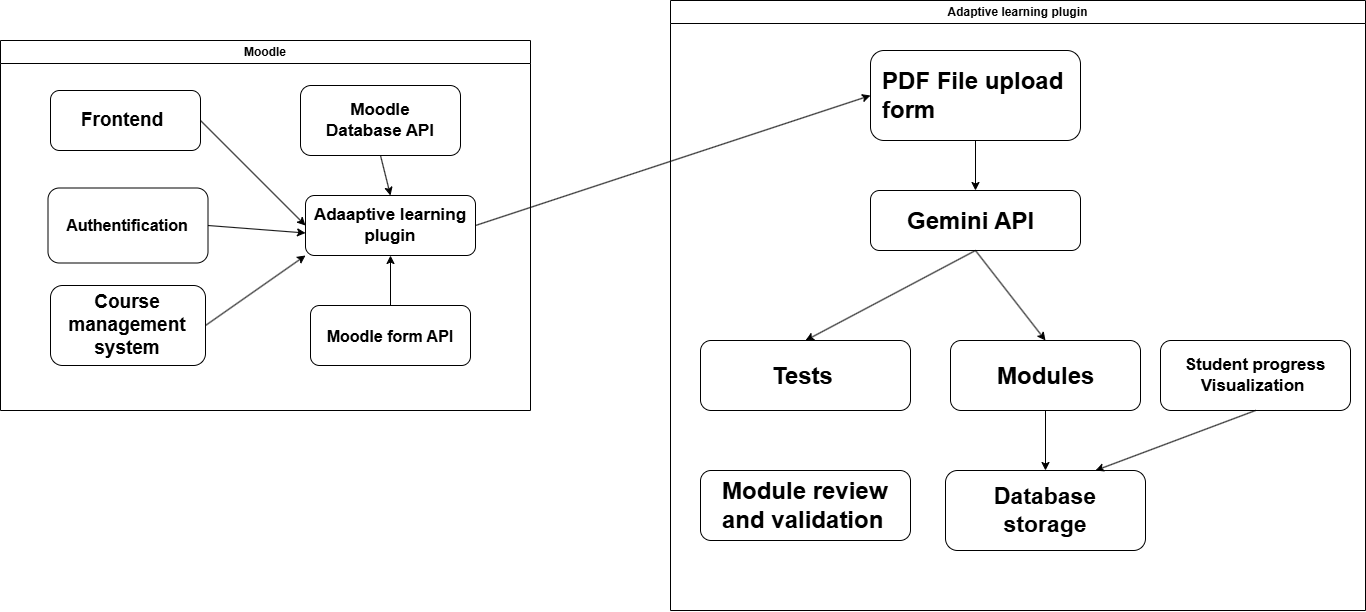
\includegraphics[width=0.8\textwidth]{images/LicentaArchitectureDiagram.png}
    \caption{Arhitectura generală a extensiei}
    \label{fig:arch_diagram}
\end{figure}

\section{Structura generală a extensiei Moodle}

\section{Configurare inițială}

\section{Definirea tabelelor din baza de date}

\section{Interfața și pagini}

\section{Comunicarea cu Gemini API}

\section{Logica de progres și note}

\section{Aspectul paginii și stilizarea}
